%File: Orr.tex
\documentclass[letterpaper]{article} % DO NOT CHANGE THIS
\usepackage{aaai2026}  % DO NOT CHANGE THIS
\usepackage{times}  % DO NOT CHANGE THIS
\usepackage{helvet}  % DO NOT CHANGE THIS
\usepackage{courier}  % DO NOT CHANGE THIS
\usepackage[hyphens]{url}  % DO NOT CHANGE THIS
\usepackage{graphicx} % DO NOT CHANGE THIS
\urlstyle{rm} % DO NOT CHANGE THIS
\def\UrlFont{\rm}  % DO NOT CHANGE THIS
\usepackage{natbib}  % DO NOT CHANGE THIS AND DO NOT ADD ANY OPTIONS TO IT
\usepackage{caption} % DO NOT CHANGE THIS AND DO NOT ADD ANY OPTIONS TO IT
\frenchspacing  % DO NOT CHANGE THIS
\setlength{\pdfpagewidth}{8.5in} % DO NOT CHANGE THIS
\setlength{\pdfpageheight}{11in} % DO NOT CHANGE THIS
%
% These are recommended to typeset algorithms but not required. See the subsubsection on algorithms. Remove them if you don't have algorithms in your paper.
\usepackage{algorithm}
\usepackage{algorithmic}
%\usepackage{amsmath}
\usepackage{amsmath,amssymb}
%
% These are are recommended to typeset listings but not required. See the subsubsection on listing. Remove this block if you don't have listings in your paper.
\usepackage{newfloat}
\usepackage{listings}
\DeclareCaptionStyle{ruled}{labelfont=normalfont,labelsep=colon,strut=off} % DO NOT CHANGE THIS
\lstset{%
	basicstyle={\footnotesize\ttfamily},% footnotesize acceptable for monospace
	numbers=left,numberstyle=\footnotesize,xleftmargin=2em,% show line numbers, remove this entire line if you don't want the numbers.
	aboveskip=0pt,belowskip=0pt,%
	showstringspaces=false,tabsize=2,breaklines=true}
\floatstyle{ruled}
\newfloat{listing}{tb}{lst}{}
\floatname{listing}{Listing}
%
% Keep the \pdfinfo as shown here. There's no need
% for you to add the /Title and /Author tags.
\pdfinfo{
/TemplateVersion (2026.1)
}

% DISALLOWED PACKAGES
% \usepackage{authblk} -- This package is specifically forbidden
% \usepackage{balance} -- This package is specifically forbidden
% \usepackage{color (if used in text)
% \usepackage{CJK} -- This package is specifically forbidden
% \usepackage{float} -- This package is specifically forbidden
% \usepackage{flushend} -- This package is specifically forbidden
% \usepackage{fontenc} -- This package is specifically forbidden
% \usepackage{fullpage} -- This package is specifically forbidden
% \usepackage{geometry} -- This package is specifically forbidden
% \usepackage{grffile} -- This package is specifically forbidden
% \usepackage{hyperref} -- This package is specifically forbidden
% \usepackage{navigator} -- This package is specifically forbidden
% (or any other package that embeds links such as navigator or hyperref)
% \indentfirst} -- This package is specifically forbidden
% \layout} -- This package is specifically forbidden
% \multicol} -- This package is specifically forbidden
% \nameref} -- This package is specifically forbidden
% \usepackage{savetrees} -- This package is specifically forbidden
% \usepackage{setspace} -- This package is specifically forbidden
% \usepackage{stfloats} -- This package is specifically forbidden
% \usepackage{tabu} -- This package is specifically forbidden
% \usepackage{titlesec} -- This package is specifically forbidden
% \usepackage{tocbibind} -- This package is specifically forbidden
% \usepackage{ulem} -- This package is specifically forbidden
% \usepackage{wrapfig} -- This package is specifically forbidden
% DISALLOWED COMMANDS
% \nocopyright -- Your paper will not be published if you use this command
% \addtolength -- This command may not be used
% \balance -- This command may not be used
% \baselinestretch -- Your paper will not be published if you use this command
% \clearpage -- No page breaks of any kind may be used for the final version of your paper
% \columnsep -- This command may not be used
% \newpage -- No page breaks of any kind may be used for the final version of your paper
% \pagebreak -- No page breaks of any kind may be used for the final version of your paperr
% \pagestyle -- This command may not be used
% \tiny -- This is not an acceptable font size.
% \vspace{- -- No negative value may be used in proximity of a caption, figure, table, section, subsection, subsubsection, or reference
% \vskip{- -- No negative value may be used to alter spacing above or below a caption, figure, table, section, subsection, subsubsection, or reference

\setcounter{secnumdepth}{0} %May be changed to 1 or 2 if section numbers are desired.

% The file aaai2026.sty is the style file for AAAI Press
% proceedings, working notes, and technical reports.
%

% Title

% Your title must be in mixed case, not sentence case.
% That means all verbs (including short verbs like be, is, using,and go),
% nouns, adverbs, adjectives should be capitalized, including both words in hyphenated terms, while
% articles, conjunctions, and prepositions are lower case unless they
% directly follow a colon or long dash
\title{Metacognitive(Metacognitive ... (Metacognitive Aesthetics) ... )): \\Implications for Coupled Human - AI systems}
\author{
    Mark Orr, Tiffany Seeley
}
\affiliations{
    Institute for Human and Machine Cognition\\
    morr@ihmc.org
}




\begin{document}

\maketitle

\begin{abstract}
Metacognitive aesthetics integrates human aesthetics theory into a human cognitive architecture (ACT-R) to derive aesthetic agents; agents who evaluate the valence of objects according to principles of aesthetic theory.  We first sandbox the theory, its basic operations and its control.  Then, we attempt to validate our theory against empirical data from the Music Streaming Sessions Dataset (MSSD). The empirical work provides first-order, provisional support for our theory.  We offer some directions for future research and potential implications for coupled human-AI systems.  
\end{abstract}

\section{Introduction}
A fundamental feature of biological agency is some capacity to sort out the valence (good/bad, useful/non-useful, safe/dangerous, etc.) of objects and situations in the world.  Early neural systems evolved to detect valence (e.g., early bilateralism was selected for as a mechanism for avoiding and approaching stimuli and contexts).  In a real sense, valence is the first semantic; it tells an agent (or reveals about an agent) what differences make a difference \cite{dennett2017bacteria}.  

We consider valence to be a first-order, general metacognitive signal.  It provides an agent with an evaluation of an object, situation, context (or similar kinds of things).  In contrast to utility or preference (derived from utility comparison), valence is about a state associated with an object, not a valuation of the consequences of action.   For the present, we are concerned specifically with aesthetic evaluation, an evaluation of how much a thing or object is liked or desired.  

Aesthetic evaluation, as we will attempt to demonstrate here, may be useful as the kernel for some classes of coupled human-AI systems.  Take recommender systems (RS), a human-AI coupling extraordinaire. 
%Recommender systems (RS) typically implement user-item pairing and similarity-based approaches to rate utility of choice items. 
Prediction and ranking are the core problems. Prediction approaches predict a user-item pair and for cases where item ratings are missing then inference is pursued to impute incomplete matrices. Ranking approaches rank top-k items rather than predicting user-item pairs. Notable RS models include Collaborative Filtering, Content-Based, Knowledge-Based and Hybrid-Based. \cite{aggarwal2016model}

For the human in such a system, the aesthetic evaluation of content is paramount and correlated with behavior ("I hate this song, lets skip it", "I don't like that actor, turn it off", "I kinda like the beat in this tune, its interesting, turn it up")  Yet, despite this somewhat obvious analysis, recommender systems are generally devoid of such insights.  We call this \textbf{\textit{poverty of the algorithm}}.  

To understand this, consider collaborative filtering and content-based approaches as a case-in-point.  Collaborative filtering (CF) derives ratings from users or items based on a neighborhood of similarities. Behavioral features are used to gain explicit ratings for example user interactivity with items such as likes, skips, dislikes, while implicit ratings may be derived from external sources.  Nearest neighbor algorithms are widely used to fit users into groups which then predict items which would commonly be liked by the group.  Content-based (CB) approaches use descriptive content attributes about items and are employed in cases where access to ratings outside individual users are unavailable. For example, a description of a previously played song may be similar to a description of another song. CB is a user-specific model-based approach such that the training data are the user’s observed items.  CB models are useful because the resultant recommendation would depend on external source of rating rather than user-specific history.  CB is a similarity-based approach and item similarity is inferred on the content descriptive attributes of the item, therefore on the basis of the attributes of the objects liked by the user. 

The poverty of the algorithm is defined by two fundamental issues: (i) lack of direct representation of internal, agent-level aesthetic evaluation, and (ii) representing (i) from a validated human cognitive model.  Our attempt at resolving this issue is to develop a metacognitive aesthetics model of how a human within a coupled human-AI system responds to stimuli in its environment.

Specifically, our approach integrates aspects of human cognitive modeling theory (using the ACT-R cognitive architecture, \cite{AndersonBothellByrneDouglassLebiereQin2004}) with a theory derived from the experimental aesthetics literature.  The latter, called the inverted-U theory, is somewhat obscure to the AI and cognitive science literatures, but is replete with solid empirical evidence from human experiments and observations \cite{berlyne1974studies,chmiel2017back}. We will describe our derivations of said theories and their integration into a human metacognitive aesthetics model in the technical section.  Following this, we will present two studies that illustrates the basic operation of our metacognitive aesthetics model in a stylized context (Study 1) and how aesthetic evaluation might be controlled given our model (Study 2).  We then provide a first-cut at empirical validation of our metacognitive aesthetics model against human observational data in the context of a real recommender system, Spotify (Study 3). 

\section{A Metacognitive Aesthetic Agent}
Let us consider a listening agent whom is presented with a stream or sequence of songs (each is a unique symbol).  For each song in the sequence, the agent reports an aesthetic evaluation while the song is presented (prior to the next song).  This is the fundamental function our metacognitive aesthetic agent: provide a metacognitive aesthetic evaluation.  

\subsection*{From Exposure to Evaluation: The Aesthetic Judgment Process}

Let $t$ denote the memory's current time, and let a \emph{chunk} $c$ be a
declarative memory unit $c = \{\,\mathrm{song}(c),\ \mathrm{val}(c)\,\}$, where
$\mathrm{song}(c)$ is a song identifier and $\mathrm{val}(c)$ is that chunk's
stored evaluation value. Because $\mathrm{val}(c)$ is a continuous quantity,
each successive exposure to a song ordinarily creates a \emph{new} chunk rather
than reinforcing an existing one (two chunks are treated as identical, and
hence reinforceable, only when every slot value matches exactly); a song $j$
may therefore have several distinct chunks $\{c : \mathrm{song}(c) = j\}$
accumulated in memory at time $t$, each with its own encoding history.

\paragraph{Base-level activation.}
Each chunk $c$ has a set of reference times $t_{c,1} < t_{c,2} < \cdots <
t_{c,n_c} < t$, one per creation or reinforcement of $c$ prior to $t$. Its
base-level activation is
\[
B(c,t) \;=\; \ln \sum_{i=1}^{n_c} \bigl(t - t_{c,i}\bigr)^{-d},
\]
where $d>0$ is the memory's decay parameter. Retrieval activation adds
independent noise,
\[
A(c,t) \;=\; B(c,t) + \varepsilon_c, \qquad
\varepsilon_c \sim \mathrm{Logistic}(0,\eta),
\]
drawn fresh at \emph{every} retrieval, with scale $\eta$ the memory's noise
parameter. (The memory's activation threshold and mismatch/similarity
parameters are disabled throughout this work, so retrieval reduces to an
unconstrained arg max over exactly-matching candidate chunks, with no minimum
activation required.)

\paragraph{Step 1 -- prediction.}
On exposure to a song $j$ at time $t$, the memory first retrieves whichever
chunk anywhere in memory currently has the highest activation, with no
constraint on which song it belongs to:
\begin{align*}
\hat c_{\mathrm{pred}}(t) &= \operatorname*{arg\,max}_{c \,\in\, M(t)} A(c,t), \\
A_{\mathrm{pred}}(t) &= A\bigl(\hat c_{\mathrm{pred}}(t),\, t\bigr),
\end{align*}
where $M(t)$ is the set of all chunks in memory at time $t$.

\paragraph{Step 2 -- actual activation.}
The memory then retrieves, among only the chunks belonging to $j$ itself, the
one with highest activation:
\begin{align*}
\hat c_j(t) &= \operatorname*{arg\,max}_{c \,\in\, M(t),\ \mathrm{song}(c) = j} A(c,t), \\
A_j(t) &= A\bigl(\hat c_j(t),\, t\bigr).
\end{align*}
This presupposes $j$ already has at least one chunk in memory. On a song's
first-ever exposure no such chunk exists, so $A_j(t)$ is undefined; a
placeholder chunk $\{j,\,0\}$ is encoded instead and no further computation is
performed on that trial (see the Bootstrap remark below).

\emph{Remark.} Steps 1 and 2 issue two separate retrievals, each drawing its
own noise realization -- so even on a trial where the predicted chunk and the
actual song's retrieved chunk coincide, $A_{\mathrm{pred}}(t)$ and $A_j(t)$ are
generically unequal.

\paragraph{Steps 3--4 -- aesthetic basis.}
The aesthetic basis of this exposure is the absolute activation gap between
prediction and actuality:
\[
x(t) \;=\; \bigl|\, A_{\mathrm{pred}}(t) - A_j(t) \,\bigr|.
\]

\paragraph{Running time-averaged aesthetic basis.}
Let $x_1, x_2, \ldots$ denote the sequence of aesthetic-basis values computed
across \emph{all} trials of the run (pooled across songs, not kept separately
per song), and let $N(t)$ index the current trial in that sequence, so that
$x_{N(t)} = x(t)$. The model maintains a single running average, in one of two
modes. Writing $K(t) = \max\bigl(1,\, N(t)-W+1\bigr)$ for the window's
starting index,
\[
\bar x(t) \;=\;
\begin{cases}
\dfrac{1}{N(t)} \displaystyle\sum_{k=1}^{N(t)} x_k, & \text{cumulative}, \\[2.2ex]
\dfrac{1}{N(t)-K(t)+1} \displaystyle\sum_{k=K(t)}^{N(t)} x_k, & \text{window},
\end{cases}
\]
updated to include $x(t)$ itself before it is used in the step below. 

\paragraph{Target width.}
A single free scaling parameter $\gamma > 0$ sets the effective target width
of the inverted-U:
\[
r(t) \;=\; \gamma\, \bar x(t).
\]
($\gamma = 1$ reduces this to using the running average directly.)

\paragraph{Evaluation.}
Provided $r(t) \neq 0$, the exposure's evaluation is a left-anchored inverted
parabola in $x(t)$ -- left root at $0$, vertex ($=1$) at $x = r(t)/2$, right
root at $x = r(t)$:
\[
\mathrm{eval}(t) \;=\; 1 - \left( \frac{2\,x(t)}{r(t)} - 1 \right)^{\!2}.
\]
When $r(t) = 0$, the evaluation -- and the encoding step below -- are skipped
for that trial.

\paragraph{Encoding.}
A new chunk $\{j,\ \mathrm{eval}(t)\}$ is learned into memory at time $t$, and
the memory's clock then advances, $t \mapsto t + \Delta t$ (a uniform tick,
$\Delta t = 1$, in the designs discussed here unless otherwise noted).

\paragraph{Bootstrap.}
A song's first exposure in a run has no prior chunk of its own, so $A_j(t)$
(Step 2) cannot be computed; the placeholder chunk $\{j,\,0\}$ noted above is
encoded in its place, and $x(t)$, $\bar x(t)$, and $\mathrm{eval}(t)$ are all
left undefined for that trial. Only a song's second and later exposures --
its repeats -- carry the full Steps 1--4 computation above.

\subsection*{Study 1: Baseline Dynamics}

\paragraph{Design.}
Study 1 exposes the agent process algorithm (described in the section above) to a stationary,
random environment: a fixed pool of songs drawn once and then sampled
uniformly at random with replacement, trial after trial, with no notion of a
controller or a realistic listener -- this is the model's own uncontrolled
behavior in isolation.

\paragraph{Parameters.}
Song pool size $10$; $200$ exposures; noise $0.25$; decay $0.5$; $\gamma=2.0$;
running average in window mode, width $20$; song sequence seeded ($\text{seed}=42$).
Of the $200$ exposures, $190$ are evaluable (each song's own first exposure is
absorbed by the bootstrap step and contributes no evaluation).

\paragraph{Results.}
Raw \texttt{evaluation} oscillates between the theoretical ceiling of $1$ and
sharp negative excursions (as low as $-3.79$, at trial $26$), consistent with
the inverted parabola's shape: unbounded below, capped at $1$ above. Its
$20$-trial rolling mean starts low (roughly $0.15$--$0.3$) through about trial
$48$, then rises sharply to about $0.65$--$0.7$ and holds within a band of
roughly $0.5$--$0.8$ for most of the remaining run -- dipping to about
$0.45$--$0.5$ near trials $140$--$160$, rising briefly to about $0.8$ near
trials $175$--$185$, and settling back to about $0.65$--$0.7$ by the run's end
(Figure~\ref{fig:design5-evaluation}). Over the full run, mean
\texttt{evaluation} is $0.609$ (s.d.\ $0.586$), median $0.774$.

\begin{figure}[t]
\centering
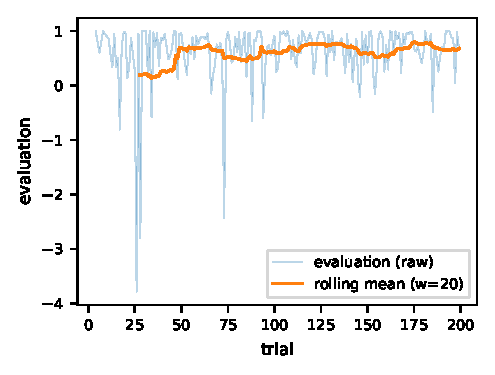
\includegraphics[width=0.8\columnwidth]{design5_evaluation_timeseries.pdf}
\caption{Study 1: raw \texttt{evaluation} per trial (light blue) and its
$20$-trial rolling mean (orange) over the $200$-exposure run.}
\label{fig:design5-evaluation}
\end{figure}

The running \texttt{time\_averaged\_aesthetic\_basis} (window mode) rises from
its initial value of about $0.33$ over the first $\sim\!10$ trials, then
fluctuates within roughly $0.6$--$1.25$ for the remainder of the run (mean
$0.993$, range $0.326$--$1.246$). Because $\gamma=2$ here, $r = \gamma \cdot
\overline x$ tracks the same shape at twice the scale, oscillating between
about $1.25$ and $2.5$ (mean $1.987$, range $0.652$--$2.492$) -- at $\gamma=1$
this line would coincide exactly with $\overline x$.
Qualitatively, both the running average and $r$ drift up and down over the
course of the run rather than converging to a constant, tracking whatever
sequence of songs the stationary environment happens to have produced
recently -- the inverted-U's target width is a moving one even in this
simplest, uncontrolled setting (Figure~\ref{fig:design5-basis}).

\begin{figure}[t]
\centering
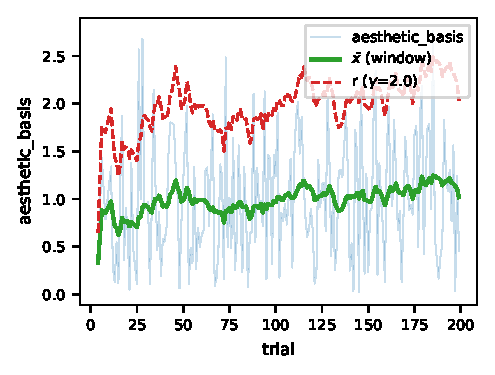
\includegraphics[width=0.8\columnwidth]{design5_time_averaged_basis.pdf}
\caption{Study 1: raw \texttt{aesthetic\_basis} per trial (light blue),
its running average $\overline x$ in window mode (green), and
$r=\gamma\cdot\overline x$ at $\gamma=2.0$ (red, dashed).}
\label{fig:design5-basis}
\end{figure}

\subsection*{Study 2: Bandit Control (Design 6)}

\paragraph{Design.}
Study 2 replaces Study 1's uniform random song draw with a controller that
chooses which song to present next, in two variants, and compares both
against an uncontrolled baseline run at otherwise identical parameters.
Algorithm C1 is a non-stationary (sliding-window) UCB bandit over the fixed
song pool, whose only signal is the \texttt{evaluation} value most recently
observed for each song -- it has no access to the memory agent's internal
state. Algorithm C2 is the same bandit augmented with privileged access to
the agent's live $r$ (which locates the inverted-U's peak at $\mathrm{aesthetic\_basis} =
r/2$): whenever $r$ shifts by more than a relative threshold between trials,
C2 resets its accumulated reward statistics outright, letting it re-adapt
immediately to a moved target rather than waiting for stale rewards to age
out of its own sliding window.

\paragraph{Parameters.}
All three conditions (uncontrolled baseline, C1, C2) share the same
environment and agent parameters: song pool size $30$; $600$ exposures; noise
$0.25$; decay $0.5$; $\gamma=2.0$; running average in window mode, width $20$;
seed $42$. Bandit-specific parameters (C1 and C2 alike): sliding window $20$,
UCB exploration constant $c=2.0$; C2's relative change-point threshold on $r$
is $0.15$. Convergence is assessed by the criterion \texttt{evaluation}
sustains at least $0.9$ for $20$ consecutive trials, with steady-state
performance then averaged over the following $100$ trials.

\emph{Caveat.} Pyactup's own activation-noise generator cannot be seeded
independently of the rest of the run, so a shared \texttt{seed} does not make
noise draws identical across the three conditions when $\text{noise}>0$; the
comparison below is therefore not a strictly matched, reproducible one, only
a single noisy realization of each condition.

\paragraph{Results.}
Neither controller ever sustains $20$ consecutive trials at
$\mathrm{evaluation} \ge 0.9$ at these settings (both convergence trial and
steady-state mean are undefined for C1 and C2 alike) -- \texttt{evaluation}'s
downside is unbounded while its upside is capped at $1$, so a strict
streak-based criterion is a demanding bar here. Median and mean
\texttt{evaluation} over the full run instead show a consistent ordering
(Table~\ref{tab:design6-comparison}).

\begin{table}[t]
\centering
\setlength{\tabcolsep}{3pt}
\begin{tabular}{lcc}
condition & median eval. & mean eval. \\
\hline
uncontrolled baseline & 0.916 & 0.800 \\
C1 (evaluation-only) & 0.962 & 0.887 \\
C2 (privileged $r$) & 0.968 & 0.916 \\
\end{tabular}
\caption{Study 2: median and mean \texttt{evaluation} over the full run,
by condition.}
\label{tab:design6-comparison}
\end{table}

C2 improves on both measures over both alternatives; C1 improves on the
uncontrolled baseline's median more than its mean, since C1's rolling-mean
trajectory tracks C2 closely for roughly the first two-thirds of the run but
then declines over its final $\sim\!150$ trials (dipping as low as
$\sim\!0.55$--$0.6$ by the run's end, versus C2 remaining mostly above
$0.85$ throughout) -- a large excursion the mean is sensitive to but the
median is not. Visually, the uncontrolled baseline sits conspicuously below
both controllers for nearly the entire run, repeatedly dipping to
$0.4$--$0.6$ where C1 and C2
mostly remain above $0.85$ (Figure~\ref{fig:design6-comparison}).

\begin{figure}[t]
\centering
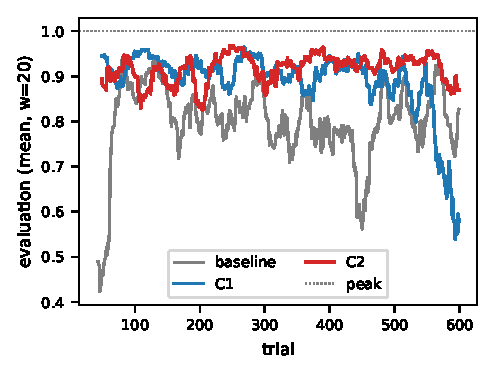
\includegraphics[width=0.8\columnwidth]{design6_evaluation_comparison.pdf}
\caption{Study 2: $20$-trial rolling-mean \texttt{evaluation} over the
$600$-exposure run for the uncontrolled baseline (gray), C1 (blue), and C2
(red).}
\label{fig:design6-comparison}
\end{figure}

C2's own observed $r$ (its privileged signal) is genuinely non-stationary
over the run (range $2.92$--$5.40$, mean $3.45$): after an initial transient
spike to its maximum of $5.40$ within the first $\sim\!30$ trials, it settles
into a repeating pattern of rise-and-fall cycles within roughly $3.0$--$4.15$
for the remainder of the run (peaks near trials $60$, $120$, $245$, $320$,
$430$, and $500$; troughs near trials $35$, $100$, $195$, $290$, $380$, and
$475$) -- direct confirmation that the inverted-U's target genuinely drifts
during the run, which is the premise C2's change-point reset is designed to
track (Figure~\ref{fig:design6-r}).

\begin{figure}[t]
\centering
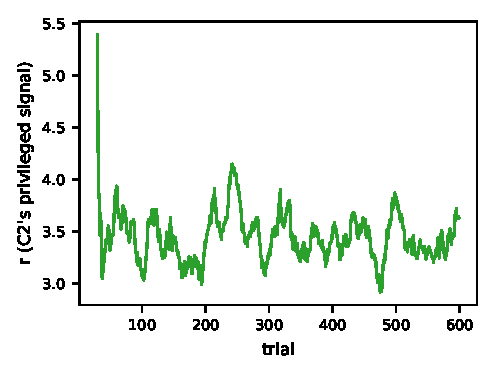
\includegraphics[width=0.8\columnwidth]{design6_c2_r_trajectory.pdf}
\caption{Study 2: C2's privileged signal $r$ over the course of the run,
showing several complete non-stationary rise-and-fall cycles.}
\label{fig:design6-r}
\end{figure}

\subsection*{Summary of Study 1 and 2}
The purpose of Study 1 and 2 were to illustrate the operation and control of our metacognitive agent in a highly stylized context.  Study 1 provides a sense of how the metacognitive aesthetic agent evaluates stimuli in an ergodic context with a small sample of songs.  We hope this provides an understanding of how the model operates and performs under such conditions.  Study 2 was designed to explore control of the metacognitive aesthetic agent's evaluations in the direction of increasing its evaluation.  The analog in a real recommender system would be to increase the aesthetic experience of the users or, put another way, to decrease the probability of disengagement with the system.  In this highly stylized example, we show that control may be possible. Together, Studies 1 and 2 provide the kinds of contexts of human-AI coupled systems to which we think our model bear fruit. The next step, an important one, was to test the predictions of our model given real data. 


\subsection*{Empirical Validation Data for Study 3}

\paragraph{Data source.}
Real listening data is drawn from the Music Streaming Sessions Dataset (MSSD;
Brost, Mehrotra \& Jehan, 2019), specifically its WSDM Cup 2019 skip-prediction
log release: daily log files of anonymized listening sessions, each row a
single track play carrying a session identifier, that play's ordinal position
within the session, the session's total length, a track identifier, a set of
graded skip indicators, and contextual fields (date, hour of day, and others
not used here). A session is defined by the source dataset as a maximal run of
plays separated by no more than 60 seconds of inactivity, truncated at a
maximum of 20 plays. Critically, session identifiers carry \emph{no listener
identity}: two sessions cannot be attributed to the same individual, even when
adjacent in time. Consequently the unit of analysis throughout this work is
the individual session, and each session is presented to its own freshly
initialized memory instance (see the agent process description elsewhere in
this manuscript); no chunk state is ever shared across sessions.

\paragraph{Base filter.}
Let a session $\sigma$ be an ordered sequence of plays $\sigma = (p_1, \ldots,
p_L)$, where $L = \mathrm{length}(\sigma)$ and $\mathrm{track}(p_i)$ is the
track identity played at position $i$. All analyses reported here first
restrict to maximal-length sessions,
\[
\mathcal S_{20} \;=\; \{\, \sigma : \mathrm{length}(\sigma) = 20 \,\},
\]
so that session length is held fixed and does not itself confound comparisons
across sessions.

\paragraph{Repeats, first occurrences, and gaps.}
For $\sigma \in \mathcal S_{20}$ and a track $j$ appearing in $\sigma$, define
its first-occurrence position
\[
\mathrm{first}(j,\sigma) \;=\; \min\{\, i : \mathrm{track}(p_i) = j \,\}.
\]
Track $j$ \emph{repeats} in $\sigma$ if it occurs at some later position $i >
\mathrm{first}(j,\sigma)$; for any such repeat occurrence, its \emph{gap} is
\[
g(i,\sigma) \;=\; i - \mathrm{first}\bigl(\mathrm{track}(p_i),\, \sigma\bigr).
\]
This matters because the agent process can only produce an
evaluation on a repeat occurrence -- a track's first play in a session has no
prior chunk of its own to compare against, and is instead absorbed by the
bootstrap step.

\paragraph{Qualifying Sessions}
\emph{Qualifying sessions} are those containing at least one repeat, with no restriction on
where that repeat falls or how far it sits from its first occurrence:
\[
\mathcal Q \;=\; \{\, \sigma \in \mathcal S_{20} : \text{some track in }
\sigma \text{ repeats} \,\}.
\]

For $\mathcal Q$, every evaluable row 
records where that repeat actually fell, as data rather than as a filter:
$\mathrm{first\_occurrence\_position}(p_i) = \mathrm{first}(\mathrm{track}(p_i),\sigma)$
and $\mathrm{repeat\_gap}(p_i) = g(i,\sigma)$ are carried alongside its
evaluation, so their relationship to outcomes can be examined directly rather
than imposed by the sampling frame. When a track repeats more than once in a
session, both quantities are computed against its true first occurrence, not
its most recent prior occurrence.

\paragraph{Sampling.}
Within the population $\mathcal Q$ )restricted to one
day's log, a simple random sample without
replacement was drawn (seeded for reproducibility); this was repeated across
several days' logs, evenly spaced across the full collection period rather
than concentrated on one day, and the resulting sessions pooled. Sample sizes
were chosen per experiment based on the per-session computational cost of the
evaluation protocol in use (Section on burn-in procedures) and are reported
alongside each result rather than fixed here.

\subsection*{Study 3: Real-Data Validation}

\paragraph{Design.}
Studies 1 and 2 exercised the agent in synthetic environments. Study 3 moves
to real listening data (session selection, above): the metacognitive aesthetic agent is
run once, single-pass, over each session in $\mathcal Q$ (session length
$20$, at least one repeat, no restriction on where it falls), with a fresh
model instance per session as before. Every evaluable row additionally
carries $\mathrm{first\_occurrence\_position}$ and $\mathrm{repeat\_gap}$
(session selection, above), and the derived binary behavioral label
\texttt{real\_skip} (\texttt{skip\_1} or \texttt{skip\_2}
$\Rightarrow 1$; else \texttt{skip\_3} or \texttt{not\_skipped}
$\Rightarrow 0$; else undefined) -- computed from the dataset's own skip
indicators.

\paragraph{Parameters.}
Five log files, evenly spaced across the collection period (2018-07-16,
07-31, 08-15, 08-28, 09-15); up to $1000$ sessions sampled per file
(seed $42$) from $\mathcal Q$ -- $4473$ sessions in total (one file supplied
only $473$, being much smaller overall than the other four), yielding
$19822$ raw evaluable rows. Model parameters at their defaults: noise
$0.25$, decay $0.5$, $\gamma=1.0$, running average in cumulative mode
(width $20$ unused in this mode), tick-based time advance.

\emph{Exclusions.} $416$ rows with an undefined \texttt{real\_skip}
(neither skip condition holds) are dropped ($19822 \to 19406$), then each
session's first evaluable trial is dropped (the same forced
$\mathrm{evaluation}=0$ artifact discussed for the synthetic studies) --
leaving $14957$ rows across $3761$ sessions for everything below.

\paragraph{Results.}
\texttt{evaluation} and \texttt{real\_skip} correlate in the theoretically
expected direction -- lower predicted evaluation associates with a higher
probability of a real skip -- though the effect is small: Pearson
$r=-0.0199$, Spearman $r=-0.0417$. Figure~\ref{fig:study3-eval} shows this
directly: binned skip rate declines fairly smoothly from about $0.57$ (at
$\mathrm{evaluation}\approx-6.7$) to about $0.49$--$0.52$ (at
$\mathrm{evaluation}\approx 0$--$1$), crossing the sample's overall skip rate
of $0.533$ around $\mathrm{evaluation}\approx -0.5$ to $-1$.

\begin{figure}[t]
\centering
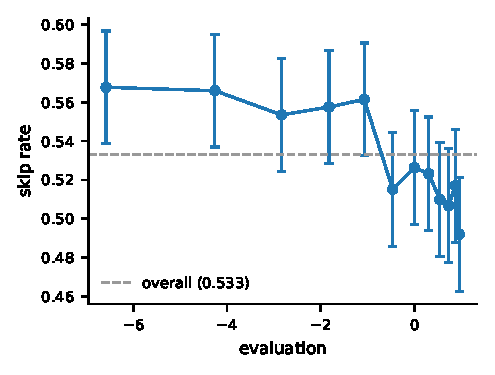
\includegraphics[width=0.75\columnwidth]{real_data_skip_rate_vs_evaluation.pdf}
\caption{Study 3: binned skip rate (with 95\% CI) against \texttt{evaluation},
restricted to its middle $90\%$ ($n=13461$).}
\label{fig:study3-eval}
\end{figure}

$\mathrm{first\_occurrence\_position}$ (mean $6.71$, median $6$, range
$1$--$19$) and $\mathrm{repeat\_gap}$ (mean $6.80$, median $6$, range
$1$--$19$) are both right-skewed (Figure~\ref{fig:study3-hist}) --
$\mathrm{repeat\_gap}$ additionally shows a pronounced even/odd alternation
(gaps of $2$, $4$, $6$, $8$ are markedly more common than $3$, $5$, $7$,
$9$), plausibly reflecting short, evenly-cycling stretches of repeated
tracks within these sessions.

\begin{figure}[t]
\centering
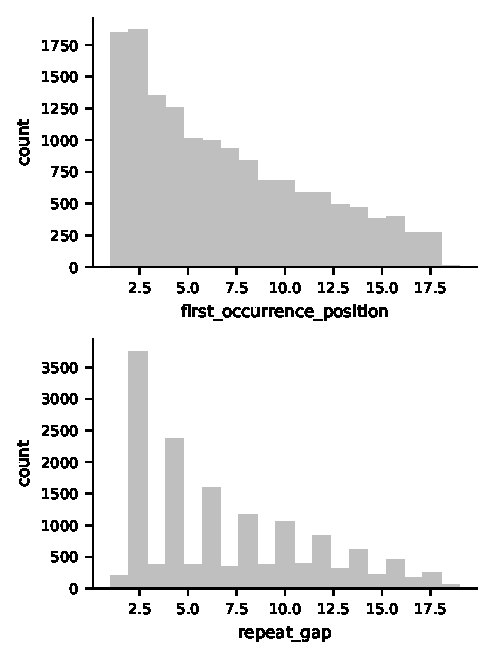
\includegraphics[width=0.9\columnwidth]{real_data_position_gap_histograms.pdf}
\caption{Study 3: distributions of $\mathrm{first\_occurrence\_position}$
(left) and $\mathrm{repeat\_gap}$ (right) across the $14957$ analyzed rows.}
\label{fig:study3-hist}
\end{figure}

Neither quantity is a strong linear predictor of outcomes, but both carry
more signal than the repeat's own raw $\mathrm{session\_position}$, which is
essentially uncorrelated with either \texttt{real\_skip} ($r=0.008$) or
\texttt{evaluation} ($r=0.007$) -- see Table~\ref{tab:study3-corr}. 

\begin{table*}[t]
\centering
\begin{tabular}{lcc}
variable & corr.\ with \texttt{real\_skip} & corr.\ with \texttt{evaluation} \\
\hline
$\mathrm{session\_position}$ & $0.008$ & $0.007$ \\
$\mathrm{first\_occurrence\_position}$ & $0.051$ & $0.047$ \\
$\mathrm{repeat\_gap}$ & $-0.045$ & $-0.041$ \\
\end{tabular}
\caption{Study 3: Pearson correlation of each position/gap variable with
\texttt{real\_skip} and \texttt{evaluation}.}
\label{tab:study3-corr}
\end{table*}

That is, it is specifically \emph{where the first play fell} and \emph{how
far apart} the two plays sit that carry a (small) relationship to outcomes 
-- not simply how late in the session the repeat itself occurs.

The binned relationships (Figure~\ref{fig:study3-gap-position}) are
non-monotonic, richer than these linear correlations alone suggest. Skip
rate against $\mathrm{repeat\_gap}$ rises from about $0.53$ (gap $\approx 2$)
to a local peak near $0.57$ (gap $\approx 4$--$8$, with a sharp dip to about
$0.45$ at gap $\approx 7$), then declines steadily to about $0.44$ at the
largest gaps ($\ge 16$ or so). Skip rate against
$\mathrm{first\_occurrence\_position}$ rises from about $0.45$ (position
$1$--$2$) to a plateau of about $0.55$--$0.59$ (positions $3$--$14$), then
drops back to about $0.50$ at the latest positions ($\approx 17$).

\begin{figure}[t]
\centering
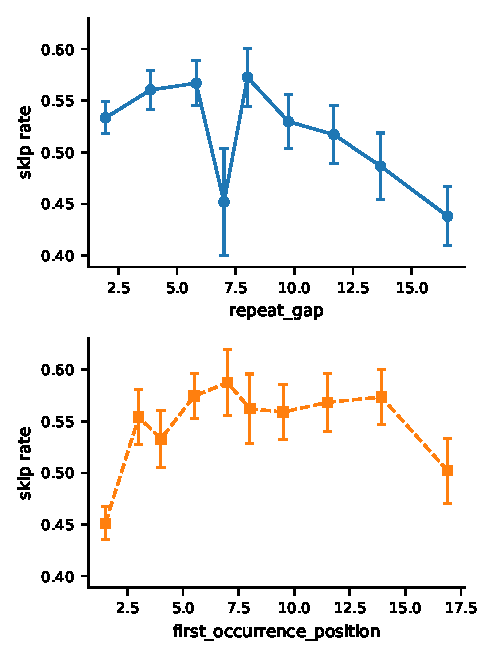
\includegraphics[width=0.95\columnwidth]{real_data_skip_rate_vs_gap_and_position.pdf}
\caption{Study 3: binned skip rate (with 95\% CI) against $\mathrm{repeat\_gap}$
(left) and $\mathrm{first\_occurrence\_position}$ (right).}
\label{fig:study3-gap-position}
\end{figure}

\paragraph{Summary of Study 3.}
The principal result of Study 3 was that the relation between the metacognitive aesthetic agent output $\mathrm{evaluation}$ and the empirical skip patterns was in the predicted direction (see Figure \ref{fig:study3-eval}).  As $\mathrm{evaluation}$ increased the probability of skipping a song decreased.  The other key result, one that may shed some light on how the aesthetic evaluation works, is that $\mathrm{repeat\_gap}$ has a non-linear relation to the probability of skipping a song.  Upon consideration, this result makes some sense given our metacognitive aesthetic agent model.  As the repeat gap increases, it is likely that a given song generates a larger value for its aesthetic basis (at the time of the repeated exposure); this may push its evaluation to the far-right of the inverted-u (parabolic) function and thus to a relatively lower evaluation value. 

In sum, the empirical data provides provisional support for the theory captured in our metacognitive aesthetic agent.

\section{Discussion}
The notion of a metacognitive aesthetic agent we put forward in this paper reflects two currents.  The first is the notion that when human cognition is an essential component of an AI system, one benefits from instantiating a model of said human in the form of a cognitive architecture.  (The literature is replete with what is a cognitive architecture, so we won't address this here.)  The other current is the fact that the AI component of human-AI coupled systems may need to deal with aesthetic processes (as human metacognitive processes) as its own metacognitive process (the AI uses the human's aesthetic signal as a metacognitive signal for control of said human).  And, to make matters more interesting, it may be the case that the human in such an arrangement is aware that the AI is using such metacognitive signals for control (reflect on your own experiences with AI systems in everyday life).  Hence the recursive title we offered for this paper.  

The theoretical underpinnings of our paper and its empirical validation are highly provision, as we suspect our reader may gather.  Let us count the ways (corse-grained).  First, the metacognitive aesthetic agent is Frankensteinian--we essentially bolted the inverted-U function from the experimental aesthetics literature onto ACT-Rs declarative memory module.  This was, in a strong sense, motivated by prior work on human memory in real contexts \cite{AndersonSchooler1991}. Here, the notion was that human memory reflects its environment in terms of what is likely to happen next.  This was the motive for our development of an aesthetic model based solely on human memory activation as opposed to more traditional features of the stimulus (e.g., stimulus familiarity, complexity, or sonic qualities).  So, we note here that the theory is very new, but was motivated by current understanding of human memory.  Second, the empirical data was truncated to sessions of length 20 (20 songs); this resulted in much of the data, for a single session, having about 1 to 2 repeats.  We mention this because it seems to limits the ecological validity of our validation design.  We would have preferred much more data per session and more sessions per person (as it was, we could not identify person and thus could not concatenate multiple sessions per person).  Third, for the validation, these data represent a mish-mash of different user experience modes: listening to one's own playlist, random shuffle, etc.  We would prefer to have control (statistical) of user experience mode. 

In closing, if our metacognitive aesthetic agent sustains further empirical scrutiny, we think the fundamental shift to the next generation of recommender systems and other human-AI coupled systems will be towards more agent-level cognition, at least in reduced-order model form, compute complexity and scaling notwithstanding.  The form of such cognitive models, we suggest provisionally, should arise from deep theoretical roots and cognitive architectures.  Non-cognitive models of human behavior (a la Centaur \cite{BinzEtal2025}) may also serve a role here, albeit without much theoretical basis.

\section{Related Work}
There have been attempts to integrate RS with common models of cognition architecture such as as ACT-R using base-level learning (BBL) approaches to model popularity and temporal drift of music genre preferences. \cite{Lex2020BLL} Some researchers proposed alternatives to conventional statistical approaches with the motivation to model human memory using Dynamically Structured Holographic Memory (DSHM) by proposing a user-based model Collaborative Filtering method. \cite{4746700}




\bibliography{aaai2026}

\end{document}
